\section{Structure Analysis}
\label{sec:3analysis}

Given the extensive analysis in Lab Report 1, which analyzed trusses in the vertical plane, this report focuses on analyzing trusses in the horizontal plane.
Three design alternatives were considered as seen in figures \ref{fig:hz1}, \ref{fig:hz2} and \ref{fig:hz3}.
Using the MATLAB finite element analysis code, maximum predicted deflections were calculated.
All results, including efficiency calculations are given in table \ref{tbl:results}.

\begin{figure}[p]
    \centering
    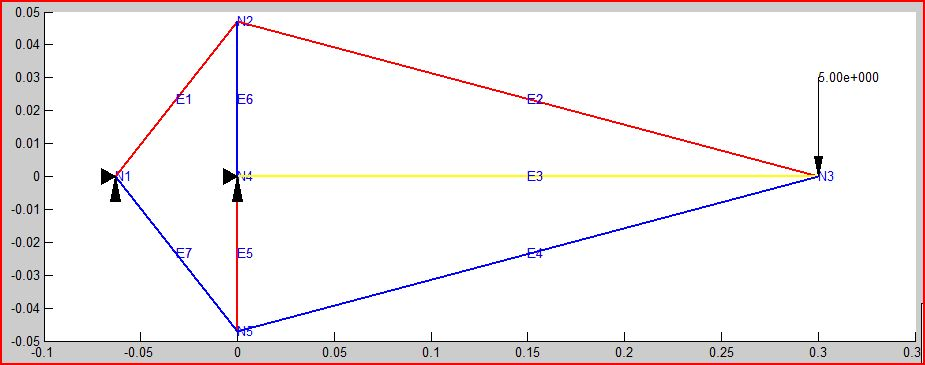
\includegraphics[width=.8\textwidth]{images/horz_truss1}
    \caption{Horizontal Truss Design 1}
    \label{fig:hz1}
\end{figure}

\begin{figure}[p]
    \centering
    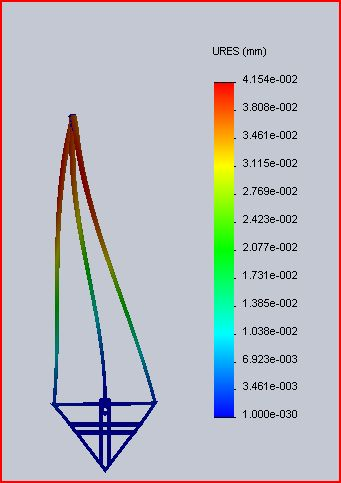
\includegraphics[width=.40\textwidth]{images/horiz_truss1_SW}
    \caption{Horizontal Truss Design 1 - SolidWorks}
    \label{fig:hz1_sw}
\end{figure}

\begin{figure}[p]
    \centering
    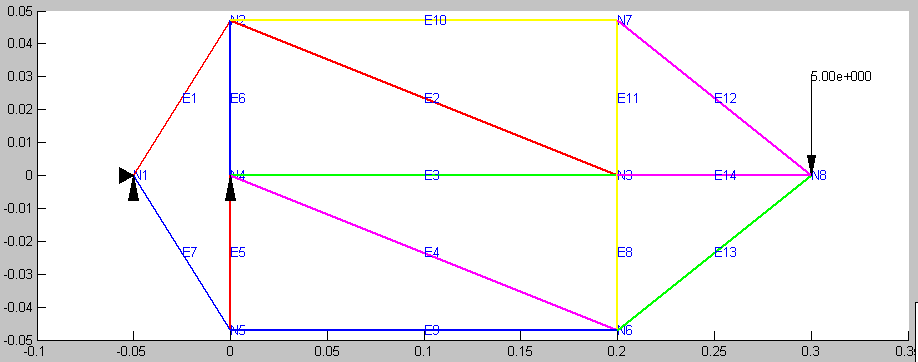
\includegraphics[width=.8\textwidth]{images/horizontal2}
    \caption{Horizontal Truss Design 2}
    \label{fig:hz2}
\end{figure}

\begin{figure}[p]
    \centering
    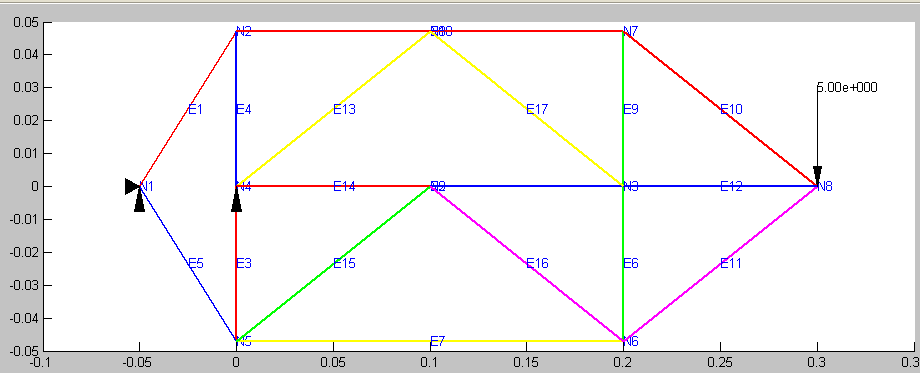
\includegraphics[width=.8\textwidth]{images/horizontal3}
    \caption{Horizontal Truss Design 3}
    \label{fig:hz3}
\end{figure}

\begin{table}[p]
	\centering
	\caption{Comparison of Designs - FE Analysis Results}
	\label{tbl:results}
	\vspace{6pt}
	\begin{tabular}{rccc}
		\toprule
		& Design 1 & Design 2 & Design 3 \\
		\midrule
		Material Length & 1.063 m & 1.675 m & 1.709 m \\
		Number of Members & 7 & 14 & 16 \\
		Mass & 71.5 g & 112.5 g & 114.9 g \\
		Max Deflection & 6.322e-005 & 5.814e-005 & 1.071e-004   \\
		Efficiency & 1,106,138 & 764,438 & 406,313 \\
		\bottomrule
	\end{tabular}
\end{table}